%================ch1======================================
\chapter{Introduction}\label{ch:ch1}

\section{A Little Intro to Bioinformatics and Genomics}
Genomics and Bioinformatics has become a buzzword in today's world of Science. About one or two decades ago, people saw biology and computer science as two different fields. One would learn about living beings and their functions whereas the other would learn about computers and underlying theories. However, at present, there seems to be a mere separation between two fields and this new-field, bioinformatics, has emerged as a combination of both Computer Science and Biology. And genomics is the study of genomes. Bioinformatics methods and tools are frequently used in genomics research, but genomics also makes use of many experimental methods. 

\section{Why Learn and Apply Genomics?} 
Bioinformatics and genomics have become an inter-disciplinary science and if you are a biologist, you will find that having knowledge in bioinformatics can benefit you immensely with your experiments and research.

A major application of bioinformatics can be found in the fields of \textbf{precision medicine}  and \textbf{preventive medicine}. Precision medicine consists of health care techniques customized for individual patients, including treatments and practices. Rather than treating or curing diseases, precision medicine focuses of developing measures to prevent diseases. Some of the diseases being focused are \textbf{influenza},\textbf{cancer}, \textbf{heart disease} and \textbf{diabetes}.


Researches are being carried out to identify genetic alterations in patients allowing scientists to come up with better treatments and even possible measures of prevention. Certain types of cancer, being caused by such genetic alterations can be identified beforehand and can be treated before the conditions get worse. \url{https://en.wikipedia.org/wiki/Genomics}


\section{What is Genome Analysis?} 
Modern biology is undergoing an historical transformation, becoming among other things increasingly data driven. A combination of statistical, computational, and biological methods has become the norm in modern genomic research. Of course this is at odds with the standard organization of university curricula, which typically focus on only one of these three subjects. It is hard enough to provide a good synthesis of computer science and statistics, let alone
to include molecular biology! Yet, the importance of the algorithms typical of this field can only be appreciated within their biological context, their results
can only be interpreted within a statistical framework, and a basic knowledge of all three areas is a necessary condition for any research project \cite{compgenome}.

Genome analysis, also known as genome mining or in silico analysis,currently constitutes an irreplaceable research tool for various aspects of microbiology\cite{ray2003}. In particular, the availability of genomes from virtually all bacterial human pathogens has opened perspectives in the fields
of diagnosis, epidemiology, pathophysiology and treatment.
A major advantage of genome sequences over phenotypic methods
is that data can rapidly be shared among scientists worldwide by being deposited in online databases and thus are easily comparable among laboratories.


\section{The Main Ideas}
The genomic sequencing era may be divided into two periods (Figure\ref{fig:sequencing_stats}). In the first decade, from 1995, when the sequencing of the \textit{Haemophilus influenzae} genome was performed \cite{ray2003} to 2005, sequencing relied on the classic Sanger method, was time- and money-consuming and was reserved to a limited number of sequencing centers world-wide. Fewer than 300 bacterial genomes were sequenced during this period (Figure\ref{fig:sequencing_stats}). Since 2005, the development of new and high-throughput sequencing methods,2 together with a steep decrease of the sequencers’ and reagents’ cost enabling many laboratories to develop their own sequencing projects, led to a striking increase in the number of sequenced genomes, approaching 6000 for the year 2013 alone. The tremendous source of information provided by genome sequences revolutionized basic aspects of microbiology. In particular,genome sizes of bacteria range from 139 kb for Candidatus Tremblaya princeps to 14 782 kb for Sorangium cellulosum (\url{http://genomesonline.org/})  \cite{ray2003}


With more than 49 000 bacterial genome sequences currently available,including those from all significant human pathogens, genomics has a significant impact on clinical microbiology and infectious diseases by enabling the development of improved diagnostic, genotyping, taxo-nomic, antibiotic and virulence marker detection tools as well as development of new culture media or vaccines. This chapter summarizes the current achievements in bacterial genomics relevant to medical microbiology.

\begin{figure}
	\centering
	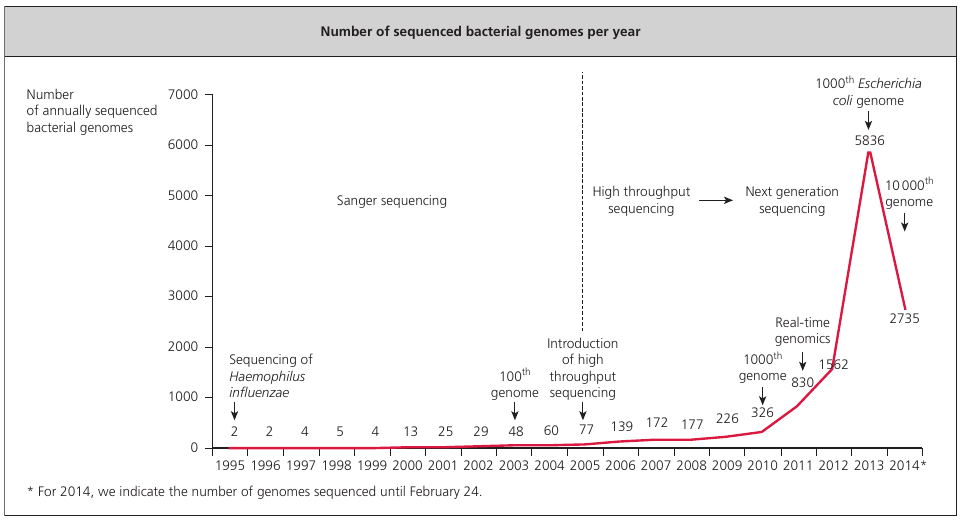
\includegraphics[width=\linewidth]{sequencing_stats}
	\caption{ Number of sequenced bacterial genomes per year.}
	\label{fig:sequencing_stats}
\end{figure} 

\section{Genomic Approaches}
The ultimate goal of genetic association studies is both to define the genetic architecture of complex traits and diseases and also to provide new insights into normal physiology and disease pathophysiology. Accomplishing that goal will require defining the causal variants that account for the observed associations, their mechanism of action, and their target genes. Success would have both near- and long-term benefits to health and science. In terms of health benefits, causal relationships between noncoding genetic variants and disease risk can be used to improve the prediction of disease onset and the design of prevention and early detection strategies. Subsequently determining the effects of causal variants on gene expression can prioritize downstream efforts to characterize causal genes and their role in disease etiology. That prioritization is particularly valuable when the target genes have an unknown function. This discovery pathway can ultimately lead to novel and potentially patient-specific therapeutic targets. In terms of scientific benefits, expanding the catalog of noncoding variants that are known to contribute to human traits is needed to determine general and transferrable principles about the genetic basis of complex human diseases. Recent conceptual and technical advances in genetics and genomics together have the potential to greatly improve our understanding of the noncoding genetic contributions to human traits. Although there are a wide variety of ways in which noncoding variants may affect phenotypes, we will focus specifically on variants that alter the activity of gene regulatory elements and, subsequently, the expression of target genes\cite{lowe2015genomic}.
